\documentclass[11pt,a4paper]{article}
\usepackage[utf8]{inputenc}
\usepackage[T1]{fontenc}
\usepackage{lmodern}
\usepackage{amsmath,amssymb,mathtools}
\usepackage[margin=2.2cm]{geometry}
\usepackage{microtype}
\usepackage{booktabs,array,tabularx}
\usepackage{enumitem}
\usepackage{xcolor}
\usepackage[most]{tcolorbox}
\usepackage{listings}
\usepackage{tikz}
\usetikzlibrary{arrows.meta,positioning,shapes.geometric}
\usepackage[colorlinks=true,linkcolor=blue!60!black,urlcolor=blue!60!black]{hyperref}
\usepackage{fancyhdr}
\setlength{\parindent}{0pt}
\setlength{\parskip}{6pt}
\renewcommand{\arraystretch}{1.25}
\pagestyle{fancy}
\fancyhf{}
\fancyhead[L]{\small GATE DA 2027 --- Artificial Intelligence}
\fancyhead[R]{\small Ramu \& Somu Notes}
\fancyfoot[C]{\thepage}

\newcommand{\Oh}{\mathcal{O}}
\newcommand{\py}[1]{\texttt{#1}}

% ---------- code listings ----------
\lstdefinestyle{py}{language=Python,basicstyle=\ttfamily\small,keywordstyle=\color{blue!60!black}\bfseries,
  commentstyle=\color{green!40!black}\itshape,stringstyle=\color{red!55!black},
  backgroundcolor=\color{gray!9},frame=single,rulecolor=\color{gray!40},breaklines=true,
  showstringspaces=false,columns=fullflexible,aboveskip=4pt,belowskip=2pt,
  xleftmargin=2pt,xrightmargin=2pt}
\lstdefinestyle{out}{basicstyle=\ttfamily\small,backgroundcolor=\color{yellow!10},frame=single,
  rulecolor=\color{orange!40},breaklines=true,showstringspaces=false,columns=fullflexible,
  aboveskip=0pt,belowskip=4pt,xleftmargin=2pt,xrightmargin=2pt}
\lstset{style=py}

% ---------- boxes ----------
\newtcolorbox{story}[1][]{breakable,enhanced,colback=yellow!10,colframe=orange!80!black,
  fonttitle=\bfseries,title={Ramu \& Somu: #1},left=6pt,right=6pt,top=4pt,bottom=4pt}
\newtcolorbox{formula}[1][Key facts]{breakable,enhanced,colback=blue!5,colframe=blue!60!black,
  fonttitle=\bfseries,title={#1},left=6pt,right=6pt}
\newtcolorbox{example}[1][Worked example]{breakable,enhanced,colback=green!6,colframe=green!45!black,
  fonttitle=\bfseries,title={#1},left=6pt,right=6pt}
\newtcolorbox{trap}{breakable,enhanced,colback=red!5,colframe=red!60!black,
  fonttitle=\bfseries,title={Common GATE traps},left=6pt,right=6pt}
\newtcolorbox{intuition}{breakable,enhanced,colback=gray!8,colframe=gray!60!black,
  fonttitle=\bfseries,title={Idea in plain words},left=6pt,right=6pt}

\lstdefinestyle{sql}{style=py,language=SQL,morekeywords={IF,EXISTS,CASCADE,REFERENCES,PRIMARY,KEY,CHECK,INTERSECT,EXCEPT,LIMIT,TRIGGER,CONSTRAINT,UNIQUE,INDEX,VIEW},
  keywordstyle=\color{blue!60!black}\bfseries,commentstyle=\color{green!40!black}\itshape}
\newcommand{\sql}[1]{\texttt{#1}}
\newcommand{\key}[1]{\underline{#1}}
\newcommand{\cl}[1]{#1^{+}}
\newcommand{\fd}{\rightarrow}
\newcommand{\R}{\mathbb{R}}
\newcommand{\E}{\mathbb{E}}
\newcommand{\bx}{\boldsymbol{x}}
\newcommand{\bw}{\boldsymbol{w}}
\newcommand{\norm}[1]{\lVert #1\rVert}
\DeclareMathOperator*{\argmin}{arg\,min}
\DeclareMathOperator*{\argmax}{arg\,max}
\newcommand{\bz}{\boldsymbol{z}}
\newcommand{\bh}{\boldsymbol{h}}
\newcommand{\indep}{\perp\!\!\!\perp}
\newcommand{\ent}{\models}
\title{\Huge\bfseries GATE DA 2027\\[4pt] \Large Artificial Intelligence\\[8pt]
\large Search, logic and reasoning under uncertainty\\
with the stories of Ramu and Somu}
\author{}
\date{}

\begin{document}
\maketitle
\thispagestyle{empty}

\begin{center}
\begin{tcolorbox}[colback=yellow!10,colframe=orange!80!black,width=0.9\textwidth,breakable]
\textbf{Ramu and Somu once more.}\\
\textbf{Ramu} asks ``but why?'' about everything. \textbf{Somu} answers with a maze, a chess board, a detective's notebook and a rainy-day sprinkler.\\[4pt]
\textbf{Syllabus covered (GATE DA, Section 7):} \emph{search:} uninformed (BFS, DFS, depth-limited, iterative deepening, uniform-cost), informed (greedy best-first, A$^*$, heuristics) and adversarial (minimax, alpha--beta pruning); \emph{logic:} propositional logic and predicate (first-order) logic; \emph{reasoning under uncertainty:} conditional independence and Bayesian networks, exact inference by variable elimination, approximate inference by sampling.\\[4pt]
\textbf{Every trace, truth-table count, unification result and probability in the worked examples was computed by code.}
\end{tcolorbox}
\end{center}

\tableofcontents
\newpage

% =====================================================================
\section{Problem Solving by Search}

\begin{story}[Finding the way out of a maze]
Ramu is in a maze and wants the exit. Somu: ``Write the maze down as a puzzle with four parts: where you \emph{start}, what \emph{moves} you may make from each place, a test for \emph{am I at the exit?}, and the \emph{cost} of each move. Then the question is only: in what order should you try the moves?''
\end{story}

\begin{formula}[Formulating a search problem]
\begin{itemize}[noitemsep]
\item \textbf{State space}: all configurations; \textbf{initial state}; \textbf{actions} available in each state; \textbf{transition model} (result of an action); \textbf{goal test}; \textbf{path cost} (sum of step costs $c(s,a,s')\ge0$).
\item A \textbf{solution} is a path from the initial state to a goal; an \textbf{optimal} solution has the least cost.
\item \textbf{Search tree}: root $=$ initial state, children $=$ successors. \textbf{Frontier} (open list) $=$ generated but not yet expanded nodes. \textbf{Graph search} also keeps an \textbf{explored} set to avoid repeating states (essential when the space has cycles).
\item Parameters: \textbf{branching factor} $b$, depth of the shallowest goal $d$, maximum depth $m$.
\item Strategies are compared by: \textbf{completeness} (finds a solution if one exists?), \textbf{optimality}, \textbf{time} and \textbf{space} (counted in nodes).
\end{itemize}
\end{formula}

% =====================================================================
\section{Uninformed (Blind) Search}

\begin{story}[Searching without a map]
``Uninformed'' means the algorithm knows only the problem's rules, nothing about \emph{which direction looks promising}. Somu compares four explorers: one explores the maze level by level (\textbf{BFS}), one runs down a corridor to its end before backing up (\textbf{DFS}), one limits how far he will run (\textbf{depth-limited}) and keeps raising the limit (\textbf{iterative deepening}), and one always extends the cheapest path so far (\textbf{uniform-cost}).
\end{story}

\begin{formula}[The strategies]
\begin{itemize}[noitemsep]
\item \textbf{Breadth-first search (BFS)}: frontier is a \textbf{FIFO queue}; expands all nodes at depth $k$ before depth $k+1$. Finds the shallowest goal.
\item \textbf{Depth-first search (DFS)}: frontier is a \textbf{LIFO stack} (or recursion); goes deep first, backtracks on dead ends.
\item \textbf{Depth-limited search (DLS)}: DFS with a depth cutoff $\ell$ (nodes at depth $\ell$ have no successors).
\item \textbf{Iterative-deepening search (IDS)}: run DLS for $\ell=0,1,2,\dots$ until a goal is found. Combines DFS's small memory with BFS's completeness and shallowest-goal property.
\item \textbf{Uniform-cost search (UCS)}: frontier is a \textbf{priority queue} ordered by path cost $g(n)$; expands the cheapest node (Dijkstra's algorithm). The goal test is applied when a node is \emph{expanded}, not when generated.
\item \textbf{Bidirectional search}: search from start and goal at once; meet in the middle.
\end{itemize}
\end{formula}
\begin{center}
\small
\begin{tabularx}{\textwidth}{>{\raggedright\arraybackslash}p{3.1cm}cccc}
\toprule
\textbf{Strategy} & \textbf{Complete?} & \textbf{Optimal?} & \textbf{Time} & \textbf{Space}\\
\midrule
BFS & yes ($b$ finite) & yes if step costs equal & $O(b^{d})$ & $O(b^{d})$\\
DFS & no (loops / infinite depth) & no & $O(b^{m})$ & $O(bm)$\\
Depth-limited & no unless $\ell\ge d$ & no & $O(b^{\ell})$ & $O(b\ell)$\\
Iterative deepening & yes & yes if step costs equal & $O(b^{d})$ & $O(bd)$\\
Uniform-cost & yes if all costs $\ge\varepsilon>0$ & yes & $O\bigl(b^{1+\lfloor C^*/\varepsilon\rfloor}\bigr)$ & same\\
Bidirectional & yes & yes (unit cost) & $O(b^{d/2})$ & $O(b^{d/2})$\\
\bottomrule
\end{tabularx}
\end{center}
\begin{formula}[Counting nodes]
BFS generates $1+b+b^2+\dots+b^{d}=\dfrac{b^{d+1}-1}{b-1}$ nodes up to depth $d$. IDS re-generates shallow levels but this is cheap, because most nodes are in the deepest level: nodes generated $=\sum_{i=0}^{d}(d+1-i)\,b^{i}$.\\
For $b=10,\ d=5$: BFS $=111\,111$; IDS $=6+50+400+3000+20\,000+100\,000=\mathbf{123\,456}$, only $11\%$ more. For $b=3,\ d=4$: BFS $=121$, IDS $=179$.
\end{formula}

\begin{center}
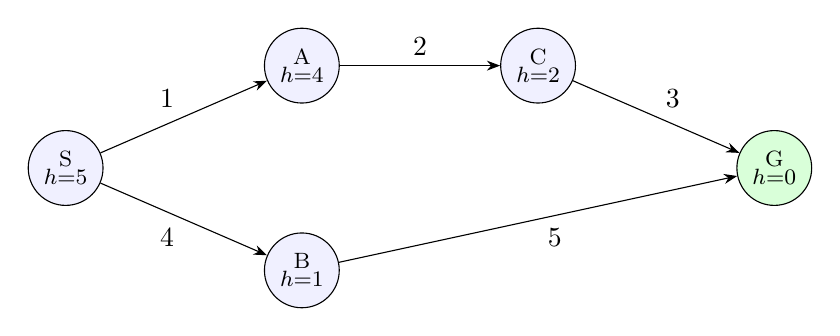
\begin{tikzpicture}[scale=1.0,>=Stealth,
 nd/.style={draw,circle,minimum size=0.95cm,inner sep=0pt,fill=blue!6,align=center,font=\footnotesize}]
\node[nd] (S) at (0,0) {S\\[-3pt]$h{=}5$};
\node[nd] (A) at (3,1.3) {A\\[-3pt]$h{=}4$};
\node[nd] (B) at (3,-1.3) {B\\[-3pt]$h{=}1$};
\node[nd] (C) at (6,1.3) {C\\[-3pt]$h{=}2$};
\node[nd,fill=green!15] (G) at (9,0) {G\\[-3pt]$h{=}0$};
\draw[->] (S)--node[above left]{1}(A); \draw[->] (S)--node[below left]{4}(B);
\draw[->] (A)--node[above]{2}(C); \draw[->] (B)--node[below right]{5}(G); \draw[->] (C)--node[above right]{3}(G);
\end{tikzpicture}
\end{center}
\begin{example}[One graph, five algorithms (start $S$, goal $G$; neighbours tried in the order $A$ then $B$)]
Step costs are on the edges; $h$ values are used later. Goal-test on expansion.
\begin{center}
\small
\begin{tabularx}{\textwidth}{>{\raggedright\arraybackslash}p{2.4cm}>{\raggedright\arraybackslash}p{4.3cm}>{\raggedright\arraybackslash}p{3.7cm}>{\raggedright\arraybackslash}X}
\toprule
\textbf{Algorithm} & \textbf{Expansion order} & \textbf{Path found} & \textbf{Cost}\\
\midrule
BFS & S, A, B, C, G & S--B--G (fewest edges) & $9$\\
DFS & S, A, C, G & S--A--C--G & $6$\\
UCS & S$(0)$, A$(1)$, C$(3)$, B$(4)$, G$(6)$ & S--A--C--G & $6$ (optimal)\\
\bottomrule
\end{tabularx}
\end{center}
BFS finds the path with the fewest \emph{edges} but not the cheapest. UCS orders by $g$: it first reaches $G$ through $B$ at cost $9$, but a cheaper copy of $G$ ($g=6$ through $C$) is pushed before $G$ is expanded, so it returns $6$.
\end{example}
\begin{trap}
(1) BFS is optimal only for \emph{equal} step costs. (2) DFS (tree search) can loop forever on cycles; graph search with an explored set fixes this but not infinite depth. (3) IDS is not wasteful: the repeated work is dominated by the last level. (4) UCS applies the goal test on \emph{expansion}. (5) The space of BFS is its major weakness ($b^d$ nodes in memory), whereas DFS needs only $O(bm)$.
\end{trap}

% =====================================================================
\section{Informed (Heuristic) Search}

\begin{story}[A compass in the maze]
Now Somu gives Ramu a compass that always shows the straight-line distance to the exit. This is a \textbf{heuristic} $h(n)$: an \emph{estimate} of the cost still to go from node $n$ to a goal. It is not exact, but it tells Ramu which corridors look promising.
\end{story}

\begin{formula}[Greedy best-first and A$^*$]
\begin{itemize}[noitemsep]
\item \textbf{Greedy best-first}: expand the node with the smallest $h(n)$. Fast when lucky, but \textbf{not optimal}, and incomplete in tree search.
\item \textbf{A$^*$ search}: expand the node with the smallest $f(n)=g(n)+h(n)$, where $g(n)$ is the cost so far and $h(n)$ the estimated cost to go. So $f$ estimates the cost of the cheapest solution \emph{through} $n$.
\item $h\equiv0$ gives uniform-cost search; $g\equiv0$ gives greedy search; unit costs and $h\equiv0$ give BFS.
\end{itemize}
\end{formula}
\begin{formula}[Admissible and consistent heuristics]
Let $h^*(n)$ be the true cheapest cost from $n$ to a goal.
\begin{itemize}[noitemsep]
\item \textbf{Admissible}: $0\le h(n)\le h^*(n)$ for all $n$ (never overestimates; ``optimistic'').
\item \textbf{Consistent (monotone)}: $h(n)\le c(n,a,n')+h(n')$ for every edge, and $h(\text{goal})=0$ (a triangle inequality).
\item \textbf{Consistent $\Rightarrow$ admissible} (not conversely).
\item \textbf{Theorem:} A$^*$ \emph{tree} search is optimal with an admissible $h$; A$^*$ \emph{graph} search is optimal with a consistent $h$. With a consistent $h$, $f$ never decreases along a path and each node is expanded at most once with its optimal $g$.
\item A$^*$ is complete (finite $b$, costs $\ge\varepsilon$), optimal, and \emph{optimally efficient} for a given heuristic, but its memory use is exponential ($O(b^{d})$ in bad cases).
\item \textbf{Dominance:} if $h_2(n)\ge h_1(n)$ for all $n$ (both admissible), $h_2$ dominates $h_1$ and A$^*$ with $h_2$ expands no more nodes. Admissible heuristics can be derived from \textbf{relaxed problems}; the maximum of two admissible heuristics is admissible.
\end{itemize}
\end{formula}

\begin{example}[A$^*$ on the graph above]
Check: $h^*(S)=6,\ h^*(A)=5,\ h^*(B)=5,\ h^*(C)=3$, and $h=(5,4,1,2)$ never exceeds them, so $h$ is admissible. Consistency: $S\to A$: $5\le1+4$; $S\to B$: $5\le4+1$; $A\to C$: $4\le2+2$; $B\to G$: $1\le5$; $C\to G$: $2\le3$. All hold, so $h$ is consistent.\\
A$^*$ expansion (ties broken by insertion order): $S\,(f=5)$, $A\,(f=1+4=5)$, $B\,(f=4+1=5)$, $C\,(f=3+2=5)$, $G\,(f=6+0=6)$. Result: path $S\!-\!A\!-\!C\!-\!G$, cost $\mathbf6$ (optimal).\\
\textbf{Greedy} best-first expands $S$, then $B$ (smallest $h=1$), then $G$: path $S\!-\!B\!-\!G$ with cost $\mathbf9$, \emph{not} optimal.
\end{example}

\subsection{Heuristics for the 8-puzzle}
\begin{formula}[Two classic admissible heuristics]
$h_1=$ number of \textbf{misplaced tiles} (not counting the blank). $h_2=$ sum of the \textbf{Manhattan distances} of the tiles from their goal squares. Both are admissible (each move shifts one tile by one square) and $h_2\ge h_1$, so $h_2$ dominates.
\end{formula}
\begin{example}[Start $\begin{smallmatrix}7&2&4\\5&\_&6\\8&3&1\end{smallmatrix}$, goal $\begin{smallmatrix}1&2&3\\4&5&6\\7&8&\_\end{smallmatrix}$]
Misplaced tiles: $7,4,5,8,3,1$, so $h_1=6$. Manhattan distances: tile $7{:}\,4$, $2{:}\,0$, $4{:}\,3$, $5{:}\,1$, $6{:}\,0$, $8{:}\,1$, $3{:}\,3$, $1{:}\,2$, sum $h_2=14$. The true optimal solution has $20$ moves (found by BFS), so $6\le14\le20$ as admissibility requires.\\
A smaller instance $\begin{smallmatrix}1&2&3\\4&\_&6\\7&5&8\end{smallmatrix}$ needs $2$ moves; $h_1=h_2=2$ (perfect).
\end{example}
\begin{formula}[Variants]
\textbf{IDA$^*$}: iterative deepening on the $f$-limit (small memory). \textbf{Weighted A$^*$}: $f=g+w\,h$ with $w>1$: faster, solution at most $w$ times optimal. \textbf{Local search} (hill climbing, simulated annealing) keeps only the current state and is used when the path does not matter; it can get stuck in local maxima.
\end{formula}
\begin{trap}
(1) Admissible does not mean consistent. (2) An overestimating heuristic can make A$^*$ return a non-optimal path. (3) $f=g+h$, not $h$ alone (that is greedy). (4) Graph-search A$^*$ needs a \emph{consistent} heuristic to stay optimal (or reopening of closed nodes). (5) The heuristic must be $0$ at goal states. (6) The larger admissible heuristic is better (dominates).
\end{trap}

% =====================================================================
\section{Adversarial Search: Games}

\begin{story}[Chess with a clever opponent]
Ramu plays Somu at a two-player board game. Ramu wants to \emph{maximise} his score, Somu wants to \emph{minimise} Ramu's score (a \textbf{zero-sum} game). ``When I plan a move,'' says Ramu, ``I must assume Somu will reply with the move that is worst for me, then I reply with my best, and so on.'' That backward reasoning through the game tree is \textbf{minimax}.
\end{story}
\begin{formula}[Minimax]
Two players \textbf{MAX} and \textbf{MIN} alternate; leaves carry utility values (from MAX's point of view). The minimax value of a node is
\[\text{MINIMAX}(n)=\begin{cases}\text{utility}(n)&\text{leaf}\\\max_{c}\text{MINIMAX}(c)&n\text{ is a MAX node}\\\min_{c}\text{MINIMAX}(c)&n\text{ is a MIN node.}\end{cases}\]
Evaluated by depth-first recursion: time $O(b^{m})$, space $O(bm)$. It is optimal against an optimal opponent and complete on a finite tree. In real games the tree is cut at a depth limit and non-terminal positions get an \textbf{evaluation function}.
\end{formula}
\begin{formula}[Alpha--beta pruning]
Carry two bounds down the tree: $\alpha=$ the best (highest) value MAX can already guarantee, $\beta=$ the best (lowest) value MIN can already guarantee. \textbf{Prune} the remaining children of a node as soon as $\alpha\ge\beta$. Alpha--beta returns \emph{exactly the same minimax value}, only faster. Pruning depends on move ordering: with the best ordering the time is $O(b^{m/2})$ (it can search twice as deep in the same time); with random ordering about $O(b^{3m/4})$; worst ordering gives no savings, $O(b^{m})$.
\end{formula}
\begin{center}
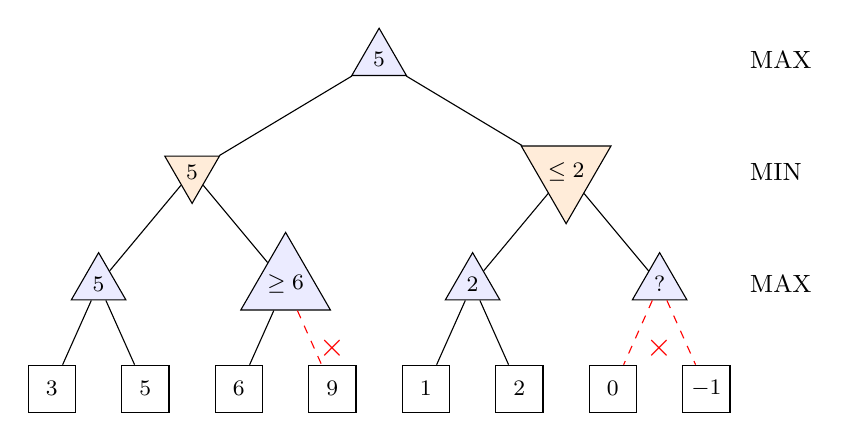
\begin{tikzpicture}[>=Stealth,scale=0.95,
 mx/.style={draw,regular polygon,regular polygon sides=3,minimum size=0.8cm,inner sep=0pt,fill=blue!8,font=\footnotesize},
 mn/.style={draw,regular polygon,regular polygon sides=3,shape border rotate=180,minimum size=0.8cm,inner sep=0pt,fill=orange!15,font=\footnotesize},
 lf/.style={draw,rectangle,minimum size=0.6cm,inner sep=0pt,font=\footnotesize}]
\foreach \i/\v in {0/3,1/5,2/6,3/9,4/1,5/2,6/0,7/-1} {\node[lf] (l\i) at (\i*1.25,0) {$\v$};}
\node[mx] (a) at (0.625,1.4) {5}; \node[mx] (b) at (3.125,1.4) {$\ge6$}; \node[mx] (c) at (5.625,1.4) {2}; \node[mx] (d) at (8.125,1.4) {?};
\node[mn] (m1) at (1.875,2.9) {5}; \node[mn] (m2) at (6.875,2.9) {$\le2$};
\node[mx] (r) at (4.375,4.4) {5};
\draw (r)--(m1); \draw (r)--(m2); \draw (m1)--(a); \draw (m1)--(b); \draw (m2)--(c); \draw (m2)--(d);
\draw (a)--(l0); \draw (a)--(l1); \draw (b)--(l2); \draw[dashed,red] (b)--(l3); \draw (c)--(l4); \draw (c)--(l5); \draw[dashed,red] (d)--(l6); \draw[dashed,red] (d)--(l7);
\node[red] at (3.75,0.55) {\large $\times$}; \node[red] at (8.125,0.55) {\large $\times$};
\node[anchor=west] at (9.2,4.4) {\small MAX}; \node[anchor=west] at (9.2,2.9) {\small MIN}; \node[anchor=west] at (9.2,1.4) {\small MAX};
\end{tikzpicture}
\end{center}
\begin{example}[Minimax and alpha--beta on the tree above (leaves left to right $3,5,6,9,1,2,0,-1$)]
Minimax: the four MAX nodes give $5,9,2,0$; the two MIN nodes give $\min(5,9)=5$ and $\min(2,0)=0$; the root gives $\max(5,0)=\mathbf5$.\\
Alpha--beta: after the first MAX node (value $5$), the MIN node has $\beta\le5$. At the second MAX node the first leaf $6\ge\beta=5$ already, so MIN will never choose this branch: the leaf $9$ is \textbf{pruned}. The MIN node returns $5$, so the root has $\alpha=5$. In the right subtree the first MAX node gives $2\le\alpha=5$, so the right MIN node can be at most $2$, never beating $5$: the whole subtree $(0,-1)$ is \textbf{pruned}. Leaves evaluated: $3,5,6,1,2$ (\textbf{5 of 8}); the answer is the same, $5$.\\
\textbf{Ordering matters:} listing the leaves as $[9,6],[5,3]$ first forces $6$ leaves to be examined for the same tree.
\end{example}
\begin{example}[A MAX--MIN tree with three leaves per MIN node]
MIN nodes with leaves $(3,12,8)$, $(2,4,6)$, $(14,5,2)$: values $3,\,2,\,2$; root $=\max=3$. Alpha--beta left to right evaluates $3,12,8,2,14,5,2$: leaves $4$ and $6$ are pruned (after reading $2\le\alpha=3$), but $14,5,2$ must all be read, because $14$ and $5$ are above $\alpha$. Seven of nine leaves are evaluated.
\end{example}
\begin{formula}[Other game ideas]
\textbf{Expectimax}: chance nodes take the \emph{expected} value of their children (dice, random opponents): e.g.\ a chance node with outcomes $3$ and $7$ at probability $\frac12$ each has value $5$. Alpha--beta cannot prune as freely there. \textbf{Evaluation function}: a weighted sum of features (material, position). \textbf{Iterative deepening} is used with time limits.
\end{formula}
\begin{trap}
(1) Pruning happens when $\alpha\ge\beta$ (including equality). (2) Alpha--beta never changes the root value. (3) Minimax assumes a \emph{perfect} opponent. (4) The number of pruned nodes depends on the ordering of children. (5) Be careful with the sign convention: leaves are values for MAX.
\end{trap}
% =====================================================================
\section{Propositional Logic}

\begin{story}[The detective's notebook]
A detective writes facts as short sentences that are either true or false: ``the butler was in the kitchen'' ($B$), ``the knife is missing'' ($K$). He combines them with ``and'', ``or'', ``not'', ``if\dots then'' and asks: \emph{given everything I know, must it follow that the cook is guilty?} That is \textbf{propositional logic}: a precise language for combining true/false statements, plus rules to decide what follows from what.
\end{story}

\subsection{Syntax and semantics}
\begin{formula}[Connectives and truth tables]
Propositions $p,q,\dots$ (atoms); connectives $\neg$ (not), $\wedge$ (and), $\vee$ (or), $\to$ (implies), $\leftrightarrow$ (iff). Precedence, high to low: $\neg,\ \wedge,\ \vee,\ \to,\ \leftrightarrow$.
\begin{center}
\begin{tabular}{cc|ccccc}
\toprule
$p$&$q$&$\neg p$&$p\wedge q$&$p\vee q$&$p\to q$&$p\leftrightarrow q$\\\midrule
T&T&F&T&T&T&T\\
T&F&F&F&T&\textbf{F}&F\\
F&T&T&F&T&T&F\\
F&F&T&F&F&T&T\\\bottomrule
\end{tabular}
\end{center}
$p\to q$ is false \emph{only} when $p$ is true and $q$ is false (a false premise makes the implication vacuously true). A \textbf{model} (interpretation) assigns T/F to every atom; with $n$ atoms there are $2^n$ models (truth-table rows) and $2^{2^n}$ distinct Boolean functions (for $n=2$: $16$).
\end{formula}
\begin{formula}[Key notions]
\begin{itemize}[noitemsep]
\item \textbf{Valid (tautology)}: true in every model. \textbf{Satisfiable}: true in at least one model. \textbf{Unsatisfiable (contradiction)}: true in none. $\alpha$ is valid iff $\neg\alpha$ is unsatisfiable.
\item \textbf{Entailment} $KB\models\alpha$: every model of $KB$ is a model of $\alpha$. \textbf{Refutation theorem:} $KB\models\alpha$ iff $KB\wedge\neg\alpha$ is unsatisfiable.
\item \textbf{Equivalent} $\alpha\equiv\beta$: same truth value in all models. \textbf{Deduction theorem:} $KB\models\alpha\to\beta$ iff $KB\wedge\alpha\models\beta$.
\item An inference procedure is \textbf{sound} if it derives only entailed sentences, and \textbf{complete} if it derives all entailed sentences.
\end{itemize}
\end{formula}
\begin{formula}[Equivalences to know]
\begin{center}
\small
\begin{tabular}{ll}
Implication & $p\to q\equiv\neg p\vee q$\\
Contrapositive & $p\to q\equiv\neg q\to\neg p$ (\emph{not} the converse $q\to p$, nor the inverse $\neg p\to\neg q$)\\
Biconditional & $p\leftrightarrow q\equiv(p\to q)\wedge(q\to p)$\\
De Morgan & $\neg(p\wedge q)\equiv\neg p\vee\neg q$; \quad $\neg(p\vee q)\equiv\neg p\wedge\neg q$\\
Double negation & $\neg\neg p\equiv p$\\
Distribution & $p\wedge(q\vee r)\equiv(p\wedge q)\vee(p\wedge r)$; \quad $p\vee(q\wedge r)\equiv(p\vee q)\wedge(p\vee r)$\\
Negated implication & $\neg(p\to q)\equiv p\wedge\neg q$\\
Exclusive or & $p\oplus q\equiv(p\vee q)\wedge\neg(p\wedge q)$
\end{tabular}
\end{center}
\textbf{Inference rules:} modus ponens $\frac{p,\ p\to q}{q}$; modus tollens $\frac{\neg q,\ p\to q}{\neg p}$; hypothetical syllogism $\frac{p\to q,\ q\to r}{p\to r}$; disjunctive syllogism $\frac{p\vee q,\ \neg p}{q}$; resolution $\frac{p\vee q,\ \neg p\vee r}{q\vee r}$.
\end{formula}
\begin{example}[Checking by truth table (all verified by program)]
\begin{itemize}[noitemsep]
\item $((p\to q)\wedge p)\to q$ is a \textbf{tautology} (modus ponens).
\item $(p\to q)\to(q\to p)$ is \textbf{not} a tautology (false when $p$ is false and $q$ is true).
\item $(p\vee q)\wedge\neg p\wedge\neg q$ is a \textbf{contradiction} ($0$ models).
\item Number of models over $\{p,q,r\}$: $p\vee q\vee r$ has $7$; $p\wedge q\wedge r$ has $1$; $(p\vee q)\wedge(\neg p\vee r)$ has $\mathbf4$; $p\to(q\to r)$ has $7$ (it is false only for $p=q=T,r=F$) and equals $(p\wedge q)\to r$. XOR and $\leftrightarrow$ have $2$ each over two atoms.
\item $\{p\to q,\ q\to r\}\models p\to r$ holds (checked over all $8$ models).
\end{itemize}
\end{example}

\subsection{Normal forms}
\begin{formula}[CNF and DNF]
A \textbf{literal} is an atom or its negation. \textbf{CNF}: a conjunction of clauses, each clause a disjunction of literals, $(l_1\vee l_2)\wedge(l_3)\wedge\cdots$. \textbf{DNF}: a disjunction of conjunctions. Every formula has an equivalent CNF and DNF. \textbf{Conversion to CNF:} (1) eliminate $\leftrightarrow$ and $\to$; (2) push $\neg$ inward with De Morgan; (3) distribute $\vee$ over $\wedge$. Example: $p\leftrightarrow q\ \equiv\ (\neg p\vee q)\wedge(\neg q\vee p)$.\\
\textbf{Horn clause}: at most one positive literal. $p_1\wedge p_2\wedge\dots\wedge p_k\to q$ is the definite-clause form $\neg p_1\vee\dots\vee\neg p_k\vee q$.
\end{formula}

\subsection{Inference algorithms}
\begin{formula}[Resolution refutation]
Resolution is \textbf{sound and refutation-complete} for CNF: to prove $KB\models\alpha$, add $\neg\alpha$ to the clauses and repeatedly resolve pairs of clauses containing complementary literals; deriving the \textbf{empty clause} $\square$ proves the entailment. If no new clauses appear and $\square$ was not derived, $KB\not\models\alpha$.
\end{formula}
\begin{example}[$KB=\{A\vee B,\ \neg A\vee C,\ \neg B\vee C\}\models C$?]
Add the negated goal $\neg C$.
\begin{enumerate}[noitemsep]
\item $\neg A\vee C$ and $\neg C$ give $\neg A$.\quad 2. $\neg B\vee C$ and $\neg C$ give $\neg B$.
\item $A\vee B$ and $\neg A$ give $B$.\quad 4. $B$ and $\neg B$ give $\square$.
\end{enumerate}
So $KB\models C$. Confirmed by truth table: the only models of $KB$ are $(A,B,C)=(T,T,T),(T,F,T),(F,T,T)$, and $C$ is true in all three.
\end{example}
\begin{formula}[Forward chaining, backward chaining, DPLL]
\begin{itemize}[noitemsep]
\item \textbf{Forward chaining} (data-driven) for definite clauses: start with the known facts; fire any rule whose premises are all known and add its conclusion; stop when the query is derived or nothing changes. Sound, complete for Horn clauses, runs in time \emph{linear} in the size of the KB.
\item \textbf{Backward chaining} (goal-driven): start from the query and work back to facts needed to prove it (like Prolog).
\item \textbf{DPLL} (SAT solver): backtracking over assignments with \textbf{unit propagation} (a clause with one unassigned literal forces it) and \textbf{pure-literal elimination}. SAT is NP-complete in general; $2$-SAT and Horn-SAT are polynomial.
\end{itemize}
\end{formula}
\begin{example}[Forward chaining]
Rules: $A\wedge B\to C$, $C\to D$, $D\wedge E\to F$. Facts: $A,B$. Fire rule 1: derive $C$. Fire rule 2: derive $D$. Rule 3 needs $E$, which is unknown. Result: $\{A,B,C,D\}$; the query $F$ is \textbf{not} entailed.
\end{example}
\begin{trap}
(1) $p\to q$ is true when $p$ is false. (2) The converse and inverse of an implication are \emph{not} equivalent to it; the contrapositive is. (3) $\neg(p\wedge q)\ne\neg p\wedge\neg q$ (De Morgan flips the connective). (4) $KB\models\alpha$ is about \emph{all} models of $KB$, not a single one. (5) Resolution proves by contradiction: remember to add $\neg\alpha$. (6) A formula can be satisfiable without being valid.
\end{trap}

% =====================================================================
\section{Predicate (First-order) Logic}

\begin{story}[When ``and, or, not'' is not enough]
Ramu wants to say ``every student in the class is clever''. With one proposition per student he would need a hundred symbols. Somu invents \textbf{variables} and \textbf{quantifiers}: $\forall x\,(\text{Student}(x)\to\text{Clever}(x))$. Now one sentence talks about \emph{everything} at once, and we can also say ``\emph{some} student scored full marks'': $\exists x\,(\text{Student}(x)\wedge\text{Full}(x))$. This richer language is \textbf{predicate (first-order) logic}.
\end{story}

\begin{formula}[Syntax]
\begin{itemize}[noitemsep]
\item \textbf{Constants} (Ramu, $0$), \textbf{variables} ($x,y$), \textbf{function symbols} (fatherOf$(x)$, $x+y$) build \textbf{terms}. \textbf{Predicates} (Loves$(x,y)$, $x<y$) applied to terms give \textbf{atomic sentences}; connectives combine them as before.
\item \textbf{Quantifiers:} $\forall x\,\varphi$ (for all), $\exists x\,\varphi$ (there exists). A variable occurrence is \textbf{bound} if inside the scope of a quantifier on it, otherwise \textbf{free}. A sentence has no free variables.
\item \textbf{Semantics:} a model has a non-empty \textbf{domain} of objects and an interpretation of every constant, function and predicate. Truth of $\forall x\,\varphi$: $\varphi$ holds for \emph{every} domain element; $\exists x\,\varphi$: for \emph{at least one}.
\end{itemize}
\end{formula}
\begin{formula}[Translating English: the two golden patterns]
\begin{center}
\begin{tabular}{ll}
All $S$ are $P$ & $\forall x\,\bigl(S(x)\to P(x)\bigr)$ \quad (use $\to$ with $\forall$)\\
Some $S$ is $P$ & $\exists x\,\bigl(S(x)\wedge P(x)\bigr)$ \quad (use $\wedge$ with $\exists$)\\
No $S$ is $P$ & $\forall x\,\bigl(S(x)\to\neg P(x)\bigr)\ \equiv\ \neg\exists x\,(S(x)\wedge P(x))$\\
Not all $S$ are $P$ & $\exists x\,\bigl(S(x)\wedge\neg P(x)\bigr)$
\end{tabular}
\end{center}
Writing $\forall x\,(S(x)\wedge P(x))$ means \emph{everything} is an $S$ and a $P$; writing $\exists x\,(S(x)\to P(x))$ is true whenever anything fails to be an $S$: both are almost always wrong translations.
\end{formula}
\begin{formula}[Quantifier rules]
\begin{itemize}[noitemsep]
\item \textbf{De Morgan for quantifiers:} $\neg\forall x\,\varphi\equiv\exists x\,\neg\varphi$; \quad $\neg\exists x\,\varphi\equiv\forall x\,\neg\varphi$.
\item Same-type quantifiers commute: $\forall x\forall y\equiv\forall y\forall x$, $\exists x\exists y\equiv\exists y\exists x$.
\item \textbf{Mixed quantifiers do not commute:} $\exists y\,\forall x\,\varphi(x,y)\ \models\ \forall x\,\exists y\,\varphi(x,y)$, but not conversely.
\item $\forall x(\varphi\wedge\psi)\equiv\forall x\,\varphi\wedge\forall x\,\psi$; \quad $\exists x(\varphi\vee\psi)\equiv\exists x\,\varphi\vee\exists x\,\psi$. But $\forall x(\varphi\vee\psi)\not\equiv\forall x\,\varphi\vee\forall x\,\psi$.
\end{itemize}
\end{formula}
\begin{example}[Evaluating sentences in finite models (checked by program)]
\textbf{Domain $\{1,2,3\}$ with $<$:}
\begin{itemize}[noitemsep]
\item $\forall x\,\exists y\,(x<y)$ is \textbf{false} (the element $3$ has nothing larger).
\item $\exists x\,\forall y\,(x<y\ \vee\ x=y)$ is \textbf{true} (take $x=1$, the minimum).
\item $\forall x\,\exists y\,(y<x)$ is \textbf{false} (nothing is below $1$).
\end{itemize}
\textbf{Order of quantifiers:} let Loves$=\{(1,2),(2,3),(3,3)\}$ on the domain $\{1,2,3\}$. $\forall x\,\exists y\,\text{Loves}(x,y)$ (everyone loves someone) is \textbf{true}; $\exists y\,\forall x\,\text{Loves}(x,y)$ (someone is loved by everyone) is \textbf{false} (nobody is loved by $1$, $2$ and $3$ together).
\end{example}

\subsection{Unification and resolution in first-order logic}
\begin{formula}[Unification]
A \textbf{substitution} $\theta$ replaces variables by terms. $\theta$ \textbf{unifies} two expressions if applying it makes them identical; the \textbf{most general unifier (MGU)} is the simplest such substitution. Algorithm: compare term by term; a variable is bound to the other term; two different constants (or function symbols) \emph{fail}; the \textbf{occurs check} forbids binding a variable to a term that contains it.
\begin{center}
\small
\begin{tabularx}{\textwidth}{>{\raggedright\arraybackslash}p{5.2cm}>{\raggedright\arraybackslash}X}
\toprule
\textbf{Pair} & \textbf{Result}\\
\midrule
$P(x,f(y))$ and $P(a,f(z))$ & $\{x/a,\ y/z\}$\\
$\text{Knows}(\text{John},x)$ and $\text{Knows}(y,\text{Mary})$ & $\{y/\text{John},\ x/\text{Mary}\}$\\
$Q(a,y)$ and $Q(x,g(x))$ & $\{x/a,\ y/g(a)\}$\\
$P(x,x)$ and $P(a,b)$ & \textbf{fails} ($x$ cannot be both $a$ and $b$)\\
$P(x,f(x))$ and $P(y,y)$ & \textbf{fails} (occurs check: $y=x$ then $x=f(x)$)\\
$x$ and $f(x)$ & \textbf{fails} (occurs check)\\
\bottomrule
\end{tabularx}
\end{center}
\end{formula}
\begin{formula}[Resolution for FOL: converting to clause form]
(1) Eliminate $\leftrightarrow,\to$. (2) Move $\neg$ inward (also through quantifiers). (3) \textbf{Standardise variables} apart. (4) \textbf{Skolemise}: replace $\exists y$ by a Skolem constant or function of the universal variables in scope: $\exists x\,P(x)\ \to\ P(c)$; $\ \forall x\,\exists y\,\text{Loves}(x,y)\ \to\ \forall x\,\text{Loves}(x,f(x))$. (5) Drop the (now all universal) quantifiers. (6) Distribute $\vee$ over $\wedge$ to get clauses.\\
Then resolve clauses whose literals unify (with the MGU), using the refutation scheme as in the propositional case. Resolution is refutation-complete for FOL, but FOL entailment is only \textbf{semi-decidable}: a proof is found if the entailment holds, but the procedure may run forever if it does not.
\end{formula}
\begin{example}[Socrates]
$KB$: $\forall x\,(\text{Human}(x)\to\text{Mortal}(x))$, $\text{Human}(\text{Socrates})$. Goal: $\text{Mortal}(\text{Socrates})$.\\
Clauses: (1) $\neg\text{Human}(x)\vee\text{Mortal}(x)$; (2) $\text{Human}(\text{Socrates})$; (3) negated goal $\neg\text{Mortal}(\text{Socrates})$.\\
Resolve (1) and (3) with $\{x/\text{Socrates}\}$: $\neg\text{Human}(\text{Socrates})$. Resolve with (2): the empty clause $\square$. Hence the goal follows. (This is generalised modus ponens.)
\end{example}
\begin{trap}
(1) With $\forall$ use $\to$; with $\exists$ use $\wedge$. (2) $\forall x\,\exists y$ is not the same as $\exists y\,\forall x$. (3) $\neg\forall x\,P(x)$ is $\exists x\,\neg P(x)$, not $\forall x\,\neg P(x)$. (4) Skolem functions depend on the universal variables in scope. (5) Unification must pass the occurs check. (6) Two distinct constants never unify. (7) First-order logic has quantification over \emph{objects} only (second-order logic would quantify over predicates).
\end{trap}
% =====================================================================
\section{Reasoning under Uncertainty}

\begin{story}[The wet-grass mystery]
One morning Ramu finds the grass wet. ``Did it rain?'' he asks. Somu: ``Maybe, or the sprinkler was on. But if I tell you the sprinkler \emph{was} on, rain becomes less likely.'' Logic cannot say ``less likely''; \textbf{probability} can. A \textbf{Bayesian network} draws who influences whom, so we can answer such questions without a huge table.
\end{story}

\subsection{Probability toolkit}
\begin{formula}[Rules you need]
Product rule $P(a,b)=P(a\mid b)P(b)$; marginalisation $P(a)=\sum_b P(a,b)$; \textbf{Bayes} $P(a\mid b)=\dfrac{P(b\mid a)P(a)}{P(b)}$; chain rule $P(x_1,\dots,x_n)=\prod_i P(x_i\mid x_1,\dots,x_{i-1})$. $A\indep B$ iff $P(A,B)=P(A)P(B)$; $A\indep B\mid C$ iff $P(A,B\mid C)=P(A\mid C)P(B\mid C)$. A full joint over $n$ Booleans needs $2^n-1$ numbers.
\end{formula}

\subsection{Bayesian networks}
\begin{formula}[Definition]
A \textbf{Bayesian network} is a directed acyclic graph (one node per variable) plus a conditional probability table (CPT) $P(X_i\mid\text{Parents}(X_i))$ per node. It represents the joint as
\[P(x_1,\dots,x_n)=\prod_{i}P\bigl(x_i\mid\text{parents}(X_i)\bigr).\]
Each Boolean node with $k$ parents needs $2^k$ numbers. \textbf{Local Markov property:} a node is independent of its non-descendants given its parents. \textbf{Markov blanket} of $X$: parents, children, and the children's other parents; given it, $X$ is independent of everything else.
\end{formula}

\begin{center}
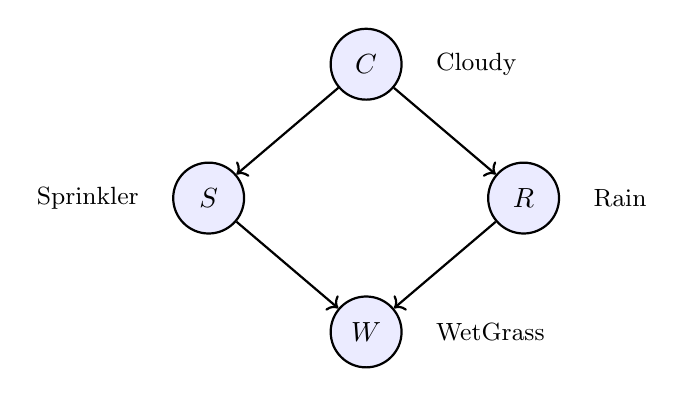
\begin{tikzpicture}[node distance=1.6cm,
 v/.style={circle,draw,thick,minimum size=9mm,fill=blue!8}]
\node[v] (C) at (0,0) {$C$};
\node[v] (S) at (-2,-1.7) {$S$};
\node[v] (R) at (2,-1.7) {$R$};
\node[v] (W) at (0,-3.4) {$W$};
\draw[->,thick] (C)--(S); \draw[->,thick] (C)--(R);
\draw[->,thick] (S)--(W); \draw[->,thick] (R)--(W);
\node[right=3mm of C,font=\small] {Cloudy};
\node[left=3mm of S,font=\small] {Sprinkler};
\node[right=3mm of R,font=\small] {Rain};
\node[right=3mm of W,font=\small] {WetGrass};
\end{tikzpicture}
\end{center}

\begin{example}[The running network]
CPTs: $P(C)=0.5$; $P(S\mid C)=0.1$, $P(S\mid\neg C)=0.5$; $P(R\mid C)=0.8$, $P(R\mid\neg C)=0.2$; $P(W\mid S,R)=0.99,\ 0.9,\ 0.9,\ 0$ for $(S,R)=(1,1),(1,0),(0,1),(0,0)$.\\
Factorisation: $P(C,S,R,W)=P(C)\,P(S\mid C)\,P(R\mid C)\,P(W\mid S,R)$.\\
\textbf{Parameters:} $1+2+2+4=\mathbf9$ numbers, against $2^4-1=\mathbf{15}$ for the full joint (the saving grows enormously for sparse graphs).\\
\textbf{One joint entry:} $P(C{=}1,S{=}0,R{=}1,W{=}1)=0.5\cdot0.9\cdot0.8\cdot0.9=\mathbf{0.324}$.\\
Marginals (by summing the joint): $P(W)=0.6471$, $P(R)=0.5$, $P(S)=0.3$.
\end{example}

\subsection{Conditional independence and d-separation}
\begin{formula}[d-separation: three basic structures]
A path is \textbf{blocked} by a set $Z$ if it contains\dots
\begin{center}
\begin{tabular}{lll}
\toprule
\textbf{Structure} & \textbf{Path} & \textbf{Blocked when}\\\midrule
Chain & $A\to B\to C$ & $B\in Z$\\
Fork (common cause) & $A\leftarrow B\to C$ & $B\in Z$\\
Collider (common effect) & $A\to B\leftarrow C$ & $B\notin Z$ \textbf{and no descendant of $B$ in $Z$}\\\bottomrule
\end{tabular}
\end{center}
$X$ and $Y$ are \textbf{d-separated} by $Z$ if every path between them is blocked; then $X\indep Y\mid Z$ holds in every distribution that factorises over the graph. Observing a collider (or its descendant) \emph{opens} the path.
\end{formula}
\begin{example}[Reading the network (numbers verified)]
\begin{itemize}[noitemsep]
\item $S\indep R\mid C$: the path $S\leftarrow C\to R$ is a fork blocked by $C$. Check: $P(S{=}1\mid C{=}1,R{=}1)=0.1=P(S{=}1\mid C{=}1)$.
\item $S\not\indep R$ marginally (path through $C$ is open): $P(S{=}1\mid R{=}1)=0.18\ne P(S{=}1)=0.30$.
\item \textbf{Explaining away.} $W$ is a collider between $S$ and $R$. Given $W{=}1$: $P(R{=}1\mid W{=}1)=0.708$. Learn also that the sprinkler was on: $P(R{=}1\mid W{=}1,S{=}1)=\mathbf{0.320}$. The sprinkler ``explains away'' the wet grass, so rain becomes less likely. Likewise $P(S{=}1\mid W{=}1)=0.430$ drops to $0.194$ once $R{=}1$ is known.
\item $C\indep W\mid\{S,R\}$ (both paths are chains blocked by $S$ and $R$).
\end{itemize}
\end{example}

\subsection{Exact inference}
\begin{formula}[Inference by enumeration]
Query $P(X\mid e)\propto\sum_{y}P(X,e,y)$ over hidden variables $y$; normalise at the end. Correct but exponential: it recomputes shared sub-sums.
\end{formula}
\begin{formula}[Variable elimination]
Keep the CPTs as \textbf{factors}. \textbf{Algorithm:} (1) restrict every factor to the observed evidence; (2) for each hidden variable $Z$ in a chosen \textbf{elimination order}: multiply all factors containing $Z$, then \textbf{sum $Z$ out}, producing a new factor; (3) multiply the remaining factors, and normalise. Factors are reused, which avoids repeated work. The cost is exponential in the size of the largest factor created, which depends on the order; the best order's largest factor has size related to the graph's \textbf{treewidth}. Finding the optimal order is NP-hard (heuristics: min-degree, min-fill). Irrelevant (barren) nodes, those that are neither the query, evidence nor their ancestors, can simply be dropped. Exact inference in general networks is NP-hard (polynomial on polytrees).
\end{formula}
\begin{example}[Variable elimination for $P(R\mid W{=}1)$]
Factors after restricting $W{=}1$: $P(C)$, $P(S\mid C)$, $P(R\mid C)$, $f(S,R)=P(W{=}1\mid S,R)$. Eliminate $S$, then $C$.\\
\textbf{Step 1.} $f_5(C,R)=\sum_S P(S\mid C)f(S,R)$:
\[f_5(0,0)=0.45,\quad f_5(0,1)=0.945,\quad f_5(1,0)=0.09,\quad f_5(1,1)=0.909.\]
(e.g.\ $f_5(0,0)=0.5\cdot0+0.5\cdot0.9=0.45$.)\\
\textbf{Step 2.} $f_6(R)=\sum_C P(C)P(R\mid C)f_5(C,R)$:
\[f_6(R{=}0)=0.5\cdot0.8\cdot0.45+0.5\cdot0.2\cdot0.09=0.189,\]
\[f_6(R{=}1)=0.5\cdot0.2\cdot0.945+0.5\cdot0.8\cdot0.909=0.4581.\]
\textbf{Step 3.} Normaliser $Z=0.189+0.4581=0.6471=P(W{=}1)$, so
\[P(R{=}1\mid W{=}1)=\frac{0.4581}{0.6471}=\mathbf{0.708}.\]
Same answer as enumeration, with smaller intermediate tables (largest factor has $2$ variables).
\end{example}

\subsection{Approximate inference by sampling}
\begin{formula}[Sampling methods]
\begin{itemize}[noitemsep]
\item \textbf{Prior (direct) sampling:} sample each variable in topological order from $P(X_i\mid\text{parents})$. Frequencies estimate probabilities; error shrinks like $1/\sqrt N$.
\item \textbf{Rejection sampling:} draw prior samples, throw away those inconsistent with the evidence, estimate from the rest. Wasteful when the evidence is rare (the accepted fraction estimates $P(e)$).
\item \textbf{Likelihood weighting:} fix the evidence variables and sample only the others; weight each sample by the product of $P(e_j\mid\text{parents})$. No rejections, but weights can become tiny when evidence is unlikely or deep in the network.
\item \textbf{Gibbs sampling (MCMC):} start from any state consistent with the evidence; repeatedly resample one non-evidence variable from $P(X\mid\text{Markov blanket})$. The samples form a Markov chain whose stationary distribution is the posterior; early samples (\emph{burn-in}) are discarded and consecutive samples are correlated.
\end{itemize}
\end{formula}
\begin{example}[Estimating $P(R{=}1\mid W{=}1)$ (simulated, $N=200\,000$)]
\begin{center}
\begin{tabular}{lc}
\toprule\textbf{Method} & \textbf{Estimate}\\\midrule
Exact (enumeration / VE) & $0.7079$\\
Rejection sampling & $0.7083$ (accepted fraction $0.6485\approx P(W)=0.6471$)\\
Likelihood weighting & $0.7084$\\
Gibbs sampling & $0.7097$\\
\bottomrule
\end{tabular}
\end{center}
All converge to the exact value; prior sampling alone estimated $P(R)\approx0.501$ (true $0.5$).
\end{example}
\begin{trap}
(1) Arrows are about the factorisation, not necessarily causation. (2) Conditioning on a \emph{collider} makes variables dependent; conditioning on a chain or fork \emph{separates} them. (3) Independence is not transitive. (4) Rejection sampling discards samples; likelihood weighting does not but uses weights. (5) Gibbs needs a Markov blanket, and burn-in. (6) Elimination order affects cost, not the answer. (7) Remember to \emph{normalise}.
\end{trap}

% =====================================================================
\section{One-page Cheat Sheet}
\begin{formula}[Search]
\begin{itemize}[noitemsep]
\item BFS: complete, optimal for unit costs, $O(b^d)$ time \emph{and} space. DFS: $O(bm)$ space, not optimal, incomplete on infinite/cyclic spaces. DLS/IDS: IDS is complete, optimal for unit cost, $O(b^d)$ time, $O(bd)$ space. UCS: expands by $g(n)$, optimal. 
\item Greedy: $f=h$ (not optimal). A*: $f=g+h$; optimal with admissible $h$ (tree search) or consistent $h$ (graph search). Consistent $\Rightarrow$ admissible, not conversely. Dominance: larger admissible $h$ expands no more nodes.
\item Minimax value by DFS; alpha-beta prunes when $\alpha\ge\beta$, same result, best case $O(b^{m/2})$.
\end{itemize}
\end{formula}
\begin{formula}[Logic and uncertainty]
\begin{itemize}[noitemsep]
\item $KB\models\alpha\iff KB\wedge\neg\alpha$ unsatisfiable; $n$ atoms $\Rightarrow$ $2^n$ models. Resolution: sound, refutation-complete. Forward chaining: linear for Horn.
\item FOL: $\forall\to$, $\exists\wedge$; $\neg\forall\equiv\exists\neg$; Skolemise $\exists$; MGU with occurs check.
\item BN: $P=\prod P(x_i\mid pa_i)$; d-separation (chain/fork blocked by observed middle; collider blocked unless observed); VE = restrict, multiply, sum out, normalise; sampling: prior, rejection, likelihood weighting, Gibbs.
\end{itemize}
\end{formula}

% =====================================================================
\section{Practice Questions}
\noindent\textbf{Answers are given right after each question.}
\begin{enumerate}[leftmargin=*,itemsep=4pt]
\item BFS with branching factor $b$ and shallowest goal at depth $d$: worst-case time? \emph{Ans:} $O(b^d)$ (space too).
\item Which uninformed strategy is complete and has space linear in depth? \emph{Ans:} none is both; IDS is complete with $O(bd)$ space (and optimal for unit costs).
\item Is DFS optimal? \emph{Ans:} no (it may find a deeper goal first).
\item UCS reduces to BFS when\dots? \emph{Ans:} all step costs are equal.
\item Define admissible heuristic. \emph{Ans:} $h(n)\le h^*(n)$ for every $n$ (never overestimates).
\item Define consistency. \emph{Ans:} $h(n)\le c(n,n')+h(n')$ for every edge; implies admissibility.
\item $h_1\le h_2$ both admissible. Which expands fewer nodes in A*? \emph{Ans:} $h_2$ (dominates).
\item Greedy best-first uses $f=$? \emph{Ans:} $h(n)$; it is not optimal.
\item A* with $h=0$ is\dots? \emph{Ans:} uniform-cost search.
\item Two admissible heuristics $h_1,h_2$: is $\max(h_1,h_2)$ admissible? \emph{Ans:} yes (and dominates both). Is $h_1+h_2$? \emph{Ans:} not necessarily.
\item Is Manhattan distance admissible for the 8-puzzle? \emph{Ans:} yes; so is the number of misplaced tiles, and Manhattan dominates it.
\item Best-case alpha-beta time with branching $b$, depth $m$? \emph{Ans:} $O(b^{m/2})$.
\item Does alpha-beta change the minimax value of the root? \emph{Ans:} no.
\item In minimax, who minimises? \emph{Ans:} the opponent (MIN); the first player (MAX) maximises.
\item When is expectimax used? \emph{Ans:} games with chance nodes; chance nodes take the expected value.
\item Number of Boolean functions of $3$ variables? \emph{Ans:} $2^{8}=256$.
\item Number of models of $p\vee q\vee r$ over $3$ atoms? \emph{Ans:} $7$.
\item Number of models of $(p\vee q)\wedge(\neg p\vee r)$ over $\{p,q,r\}$? \emph{Ans:} $4$.
\item Is $(p\to q)\to(q\to p)$ valid? \emph{Ans:} no.
\item Contrapositive of $p\to q$? \emph{Ans:} $\neg q\to\neg p$ (equivalent).
\item Negate $\forall x\,\exists y\,\text{Loves}(x,y)$. \emph{Ans:} $\exists x\,\forall y\,\neg\text{Loves}(x,y)$.
\item Translate ``Every student likes some course''. \emph{Ans:} $\forall x\,(\text{St}(x)\to\exists y\,(\text{Co}(y)\wedge\text{Likes}(x,y)))$.
\item MGU of $\text{Knows}(\text{John},x)$ and $\text{Knows}(y,\text{Mary})$? \emph{Ans:} $\{y/\text{John},\,x/\text{Mary}\}$.
\item Does $P(x,x)$ unify with $P(a,b)$? \emph{Ans:} no.
\item Does $x$ unify with $f(x)$? \emph{Ans:} no (occurs check).
\item Skolemise $\forall x\,\exists y\,\text{Loves}(x,y)$. \emph{Ans:} $\forall x\,\text{Loves}(x,f(x))$.
\item Forward chaining with $A\wedge B\to C$, $C\to D$, facts $A,B$: derived set? \emph{Ans:} $\{A,B,C,D\}$.
\item In the wet-grass network, parameters needed? \emph{Ans:} $9$ (vs $15$).
\item $P(C{=}1,S{=}0,R{=}1,W{=}1)$? \emph{Ans:} $0.324$.
\item Are $S$ and $R$ independent given $C$? \emph{Ans:} yes (fork blocked).
\item Are $S$ and $R$ independent given $W$? \emph{Ans:} no (collider observed); explaining away.
\item $P(R{=}1\mid W{=}1)$? \emph{Ans:} $0.708$.
\item $P(R{=}1\mid W{=}1,S{=}1)$? \emph{Ans:} $0.320$.
\item Which sampling method rejects samples? \emph{Ans:} rejection sampling.
\item Which method weights samples by evidence likelihood? \emph{Ans:} likelihood weighting.
\item Gibbs sampling resamples a variable from its distribution given\dots? \emph{Ans:} its Markov blanket.
\item Is the order of variable elimination relevant for correctness? \emph{Ans:} no, only for efficiency.
\end{enumerate}

\vspace{4mm}
\begin{intuition}[How to study this section]
Draw a search tree by hand for every algorithm until you can predict the expansion order. Practise translating English into logic with the two patterns until it is automatic. For networks, always write the factorisation first, then decide which variables to eliminate. Redo the explaining-away numbers once with pencil and paper: if you can reproduce $0.708$ and $0.320$, you understand the whole chapter.
\end{intuition}

\end{document}
